\section{Dimensionality Reduction}
- Summarise observed high-dimensional data points to low-dimensional vectors\\
- Avoid curse of dimensionality (Distance-based methods suffer with high dim)\\
- Reduce time/mem needed\\
- Allows visualisation (2D/3D)\\
- Reduce noise\\
\subsection*{Approaches}
- Feature selection (select subset of features)\\
(brute-force / greedy search)\\\\
- Feature Extraction\\
\textbf{Learn} k \textbf{new} features from original d features to 
represent each data instance.\\
--Linear combination of original features, e.g. (PCA)
\subsection*{Principal Component Analysis}
Algorithm:\\
1) Centering data points s.t. mean is 0\\
2) Compute sample covariance matrix\\
\[\tilde{\Sigma} = \frac{1}{N-1}\sum^N_{i=1}\mathbf{x}_i\mathbf{x}_i^T\]
Which is equavalent to:
\[\tilde{\Sigma} = \frac{1}{N-1}X^TX\]

3) Compute eigenvectors of $\tilde{\Sigma}$, $\{\mathbf{u}_1,\mathbf{u}_2,...,\mathbf{u}_d\}$
which are sorted based on their eigenvalues in non-increasing order,
i.e., $\lambda_1 \geq \lambda_2 \geq ... \geq \lambda_d$\\
4) Select first k eigenvectors to construct principal components\\
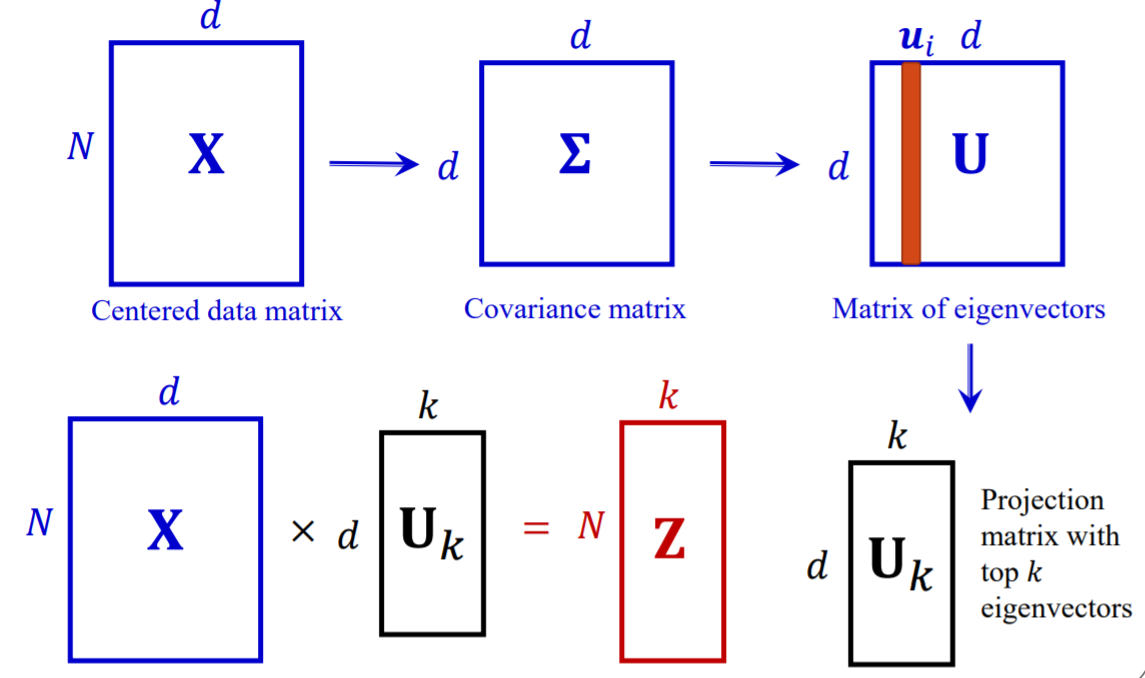
\includegraphics[width=\linewidth]{fig/pca1.PNG}
\subsection*{Computing Eigenvalues/ Eigenvectors}
With the covariance matrix:
\[\tilde{\Sigma} = \frac{1}{N-1}X^TX\]

Define a d-by-d square matrix A, such that
\[A = X^TX\]
Obtain eigenvectors and eigenvalues for A by performing SVD on X\\
As A is positive semidefinite, all eigenvalues are non-negative

\subsection*{Singular Value Decomposition (SVD)}
The SVD of X (N-by-d) has the following form:
\[X = VDU^T\]
Therefore,
\[A = X^TX = (VDU^T)^TVDU^T\]
\[A = UD^TV^TVDU^T\]
$V^TV = I$,
\[A = UD^TDU^T\]
Denoting $\bar{D} = D^T D$,
\[A = U\bar{D}U^T\]
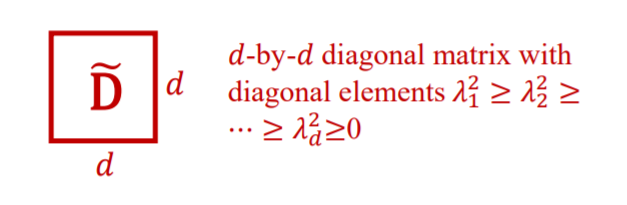
\includegraphics[width=\linewidth]{fig/pca2.PNG}
$U^TU = I$,
\[AU = U\bar{D}, \text{or }AU = \bar{D}U\]
Therefore, each column of U is an eigenvector of A, $\bar{D}$
is the square matrix where the diagonal values correspond to the eigenvalues.
